\documentclass[11pt]{beamer}
\usepackage[utf8]{inputenc}

\usetheme{Boadilla}
\usecolortheme{dolphin}

\usepackage{color,soul}
\usepackage{multicol}
\usepackage{multirow}
\usepackage{amsmath}
\usepackage{amsfonts}
\usepackage{amssymb}
\usepackage{algpseudocode} % uses algorithmicx package automatically
\usepackage{mathrsfs}
\usepackage{graphicx}
\usepackage{tikz}
\usetikzlibrary{calc}
\usepackage{pgfplots}
\usepackage{subcaption}

\begin{document}
\begin{frame}
  
\begin{figure} 
  \centering
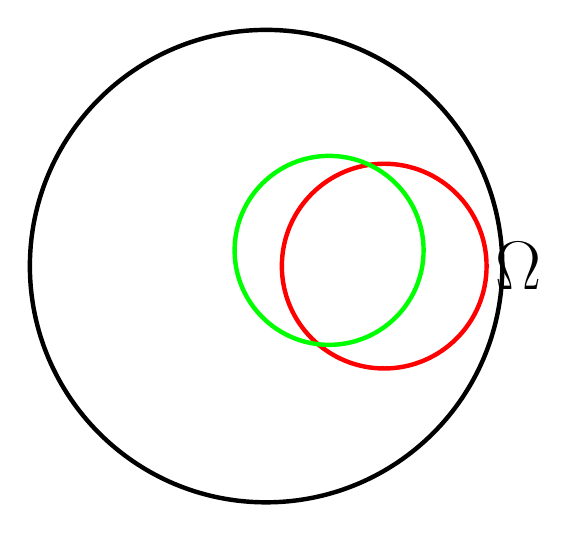
\begin{tikzpicture}
  \draw[ultra thick] (0,0) circle [radius=3];
  \node at (3.2,0) {\Huge $\Omega$};

  \onslide<2>{
      \draw[red,ultra thick] (1.5,0) circle [radius=1.3];
  }
  \onslide<3>{
      \draw[green,ultra thick] (0.8,0.2) circle [radius=1.2];
  }
\end{tikzpicture}
\end{figure}
\end{frame}

\begin{frame}
\begin{figure} 
  \centering
  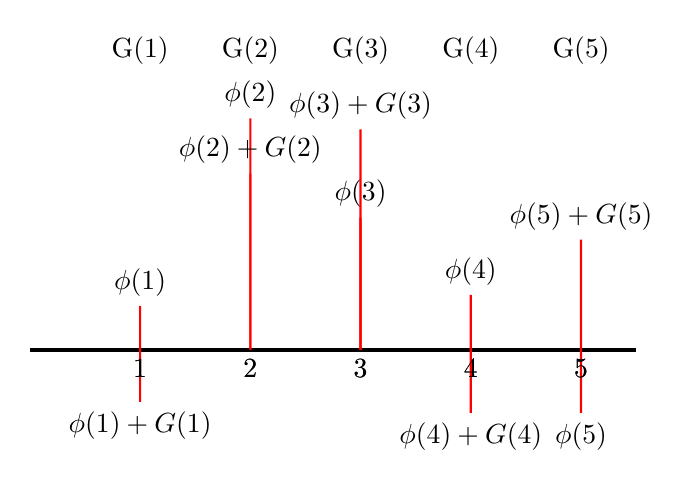
\begin{tikzpicture}[scale=0.7]
      \path[draw,black,ultra thick] (0,0)--(11,0);
      \onslide<1-2>{
        \node[above] (p1) at (2,0.8) {$\phi(1)$};
        \path[draw,red,thick] (2,0) -- (p1);
        \node[below] at (2,0) {$1$};

        \node[above] (p2) at (4,4.2) {$\phi(2)$};
        \path[draw,red,thick] (4,0) -- (p2);
        \node[below] at (4,0) {$2$};

        \node[above] (p3) at (6,2.4) {$\phi(3)$};
        \path[draw,red,thick] (6,0) -- (p3);
        \node[below] at (6,0) {$3$};

        \node[above] (p4) at (8,1.0) {$\phi(4)$};
        \path[draw,red,thick] (8,0) -- (p4);
        \node[below] at (8,0) {$4$};

        \node[above] (p5) at (10,-2.0) {$\phi(5)$};
        \path[draw,red,thick] (10,0) -- (p5);
        \node[below] at (10,0) {$5$};
      }
      \onslide<2>{
        \node[above] at (2,5) {G(1)};
        \node[above] at (4,5) {G(2)};
        \node[above] at (6,5) {G(3)};
        \node[above] at (8,5) {G(4)};
        \node[above] at (10,5) {G(5)};
      }
      \onslide<3->{
        \node[above] (p1) at (2,-1.8) {$\phi(1)+G(1)$};
        \path[draw,red,thick] (2,0) -- (p1);
        \node[below] at (2,0) {$1$};

        \node[above] (p2) at (4,3.2) {$\phi(2)+G(2)$};
        \path[draw,red,thick] (4,0) -- (p2);
        \node[below] at (4,0) {$2$};

        \node[above] (p3) at (6,4.0) {$\phi(3)+G(3)$};
        \path[draw,red,thick] (6,0) -- (p3);
        \node[below] at (6,0) {$3$};

        \node[above] (p4) at (8,-2.0) {$\phi(4)+G(4)$};
        \path[draw,red,thick] (8,0) -- (p4);
        \node[below] at (8,0) {$4$};

        \node[above] (p5) at (10,2.0) {$\phi(5)+G(5)$};
        \path[draw,red,thick] (10,0) -- (p5);
        \node[below] at (10,0) {$5$};
      }
  \end{tikzpicture}
  
\end{figure}  
\end{frame}

\end{document}
